
\section{Theorie}
\label{sec:Theorie}

Beugung ist eine typische Welleneigenschaft. Man spricht von Beugung an einem Hindernis, wenn ein Welle beim Passieren ihre Ausbreitungsrichtung verändert. Gleichzeitig kommt es zur Interferenz also zur Überlagerung von Wellen. Die Intensität der Welle hinter dem Hindernis in einem bestimmten Abstand wird Beugungsfigur genannt. Eine mögliche Erklärung für Beugung liefert das Huygenssche Prinzip. Dieses besagt, das eine Welle sich in jedem Punkt der Welle wie eine Kugelwelle ausbreitet und die Superposition dieser die Welle ergeben. Die auslaufende Kugelwelle ist proportional zu $\exp(i (k r -w t+\varphi))/r$, wobei $k$ die Wellenzahl, $r$ der Abstand zum Ausgangspunkt der Kugelwelle, $w$ die Kreisfrequenz der Welle und $t$ die Zeit ist. Es wird besonders zwischen zwei verschiedenen Näherungen unterschieden: der Fresnel-Beugung im nahem Bereich und der Fraunhofer-Beugung im fernem Bereich. Im Folgendem wird nur die Fraunhofer-Beugung betrachtet.
\begin{figure}
	\centering
	\caption{Exemplarische Darstellung der Fresnel- und Frauenhoferbeugung an einer Blende \cite{V406}.}
	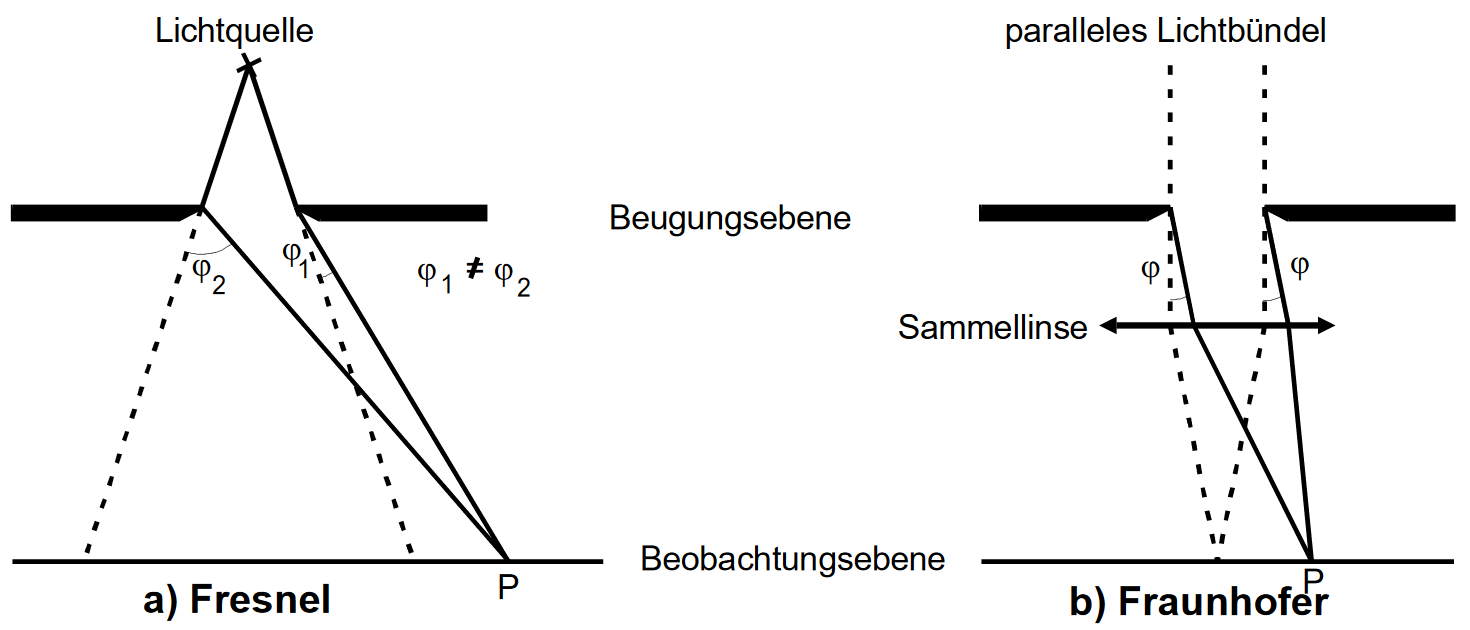
\includegraphics[width=\linewidth-150pt,height=\textheight-150pt,keepaspectratio]{content/images/FresnelFrauenhoferBeugung.png}
	\label{fig:FFB}
\end{figure}

\subsection{Beugung von kohärenten Wellen an einer Blende}

Im Folgendem wird zur Vereinfachung davon ausgegangen, dass eine kohärente und monochromatische Welle homogener Intensität senkrecht auf die Öffnung einer Blende trifft, also dass die Welle an jeder Stelle der Öffnung die selbe Phase $\varphi$, Amplitude $A$ und zusätzlich gleiche Wellenzahl $k$ besitzt (entspricht Fraunhofer-Näherung). Nach dem Huygensschen Prinzip ergibt sich dann durch Summation über alle Amplituden der Kugelwellen für die Welle $\psi$ hinter der Öffnung
\begin{equation}
	\psi = A \sum \limits_j \frac{\exp(i (k r_j -w t+\varphi))}{r_j}= \int_{\mathbb{R}^2} F(x, y) \frac{\exp(i (k |\vec{a}_0-\vec{x}| -w t+\varphi))}{|\vec{a}_0-\vec{x}|} \diff x \diff y,\label{lang}
\end{equation}
wobei $F(x, y)$ die Blendenfunktion, $\vec{x}=(x,y,0)^\text{T}$ eine Position auf der Blende und $\vec{a}_0=(a_1,a_2,a_3)^\text{T}$ die Position eines Punktes hinter der Blende ist.
Die Blendenfunktion $F(x,y)$ ist gleich Eins für die $(x, y)$ an denen die Blende durchlässig ist und ansonsten gleich Null. Nun ist jedoch keine allgemeine Stammfunktion von \eqref{lang} bekannt. Deswegen wird die Näherung $|\vec{a}_0-\vec{x}| \approx |\vec{a}_0|- \hat{\vec{a}_0} \vec{x}$ und $1/|\vec{a}_0-\vec{x}|=1/\vec{a}_0 $ für $|\vec{a}_0|\gg |\vec{x}|$ verwendet, wobei $\hat{\vec{a}_0}$ der Einheitsvektor in Richtung $\vec{a}_0$ ist. Dies entspricht der Fraunhofer-Näherung. Durch Einsetzen und Umformen ergibt sich bei einen festen Abstand $|\vec{a}_0|$ zur Blende
\begin{equation}
	\psi = C \int_{\mathbb{R}^2} F(x,y) \exp\left(-i k \hat{\vec{a}_0} \vec{x}\right) \diff x \diff y, \label{eq:Integral}
\end{equation}
mit der Konstanten $C$ bezüglich der Richtung von $\vec{a}_0$, was einer Fouriertransformation der Blendenfunktion entspricht.

\subsection{Beugung von kohärenten Wellen an einem Einzel bzw. N-fach Spalt}
\begin{figure}
	\centering
	\caption{Skizze von einem Einzelspalt \cite{V406}.}
	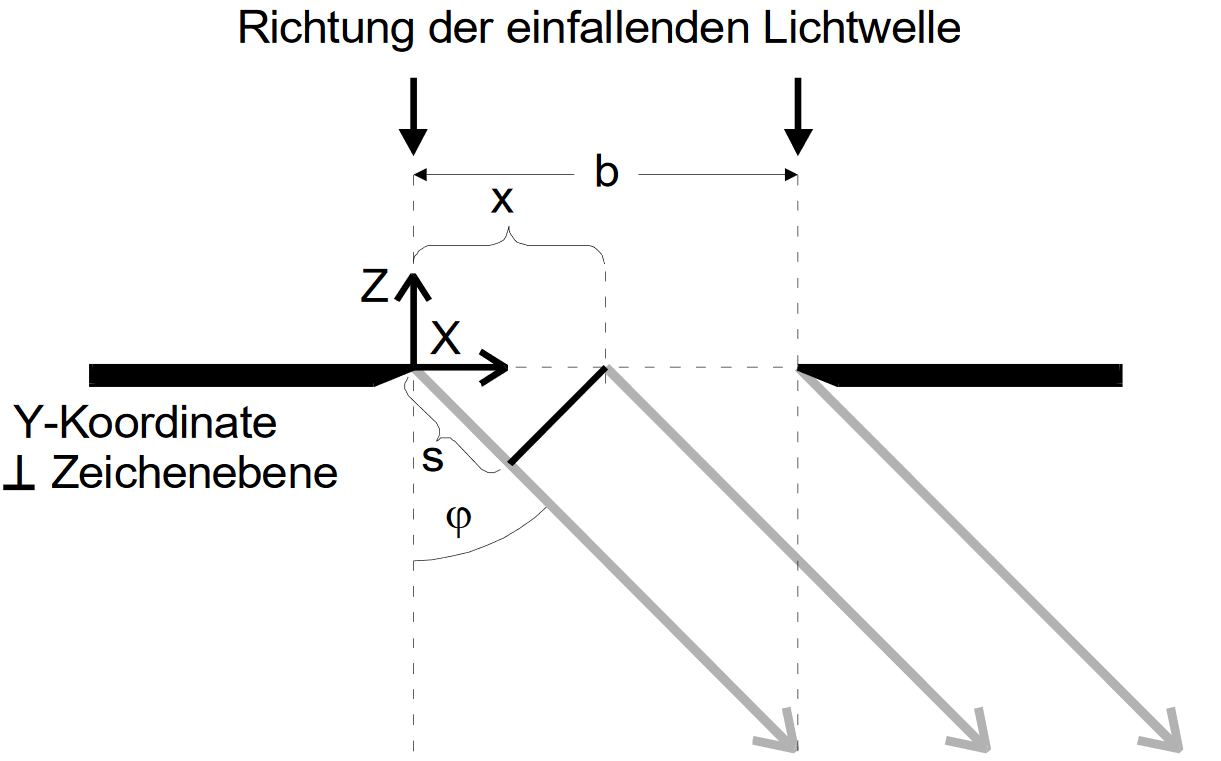
\includegraphics[width=\linewidth-150pt,height=\textheight-150pt,keepaspectratio]{content/images/Einzelspalt.png}
	\label{fig:Einzel}
\end{figure}

Für eine vorgegebene Blendenfunktion lässt sich das Integral in \eqref{eq:Integral} berechnen. Im Fall eines Einzelspalts der Breite $b$ in Richtung der $x$-Achse ergibt sich
\begin{equation}
	\psi_1 = 2 \pi C a \delta\left(k \frac{a_2}{|\vec{a}_0|}\right) \frac{\sin\left(\frac{1}{2} k \frac{a_1}{|\vec{a}_0|} b\right)}{\frac{1}{2} k \frac{a_1}{|\vec{a}_0|} b} = C' a \delta(k \sin(\theta)) \frac{\sin(\eta)}{\eta}
\end{equation} 
mit 
\begin{equation}
	\eta = \frac{1}{2} \sin(\varphi) k b .
\end{equation}
Daraus folgt für die Intensität hinter dem Einzelspalt in Abhängigkeit von $\varphi$
\begin{equation}
	I_1 \propto \frac{\sin^2(\eta)}{\eta^2}\text{.}
\end{equation}
%Diese ist in Abbildung \ref{fig:Int} aufgetragen, wobei für die Wellenlänge $\lambda=2\pi/k$ gilt.
%\begin{figure}
%	\centering
%	\caption{Darstellung der Intensitätsverteilung an einem Einzelspalt \cite{V406}.}
%	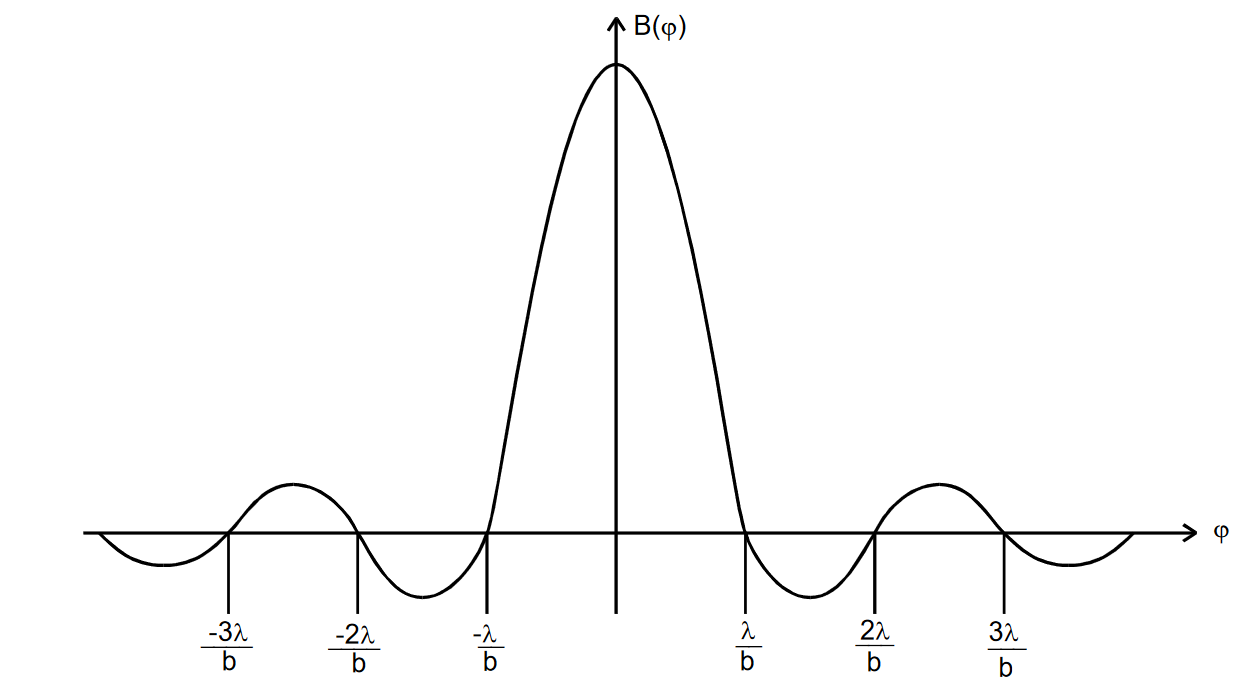
\includegraphics[width=\linewidth-70pt,height=\textheight-70pt,keepaspectratio]{content/images/Int.png}
%	\label{fig:Int}
%\end{figure}
\begin{figure}
	\centering
	\caption{Skizze von einem Doppelspalt ($N=2$) \cite{V406}.}
	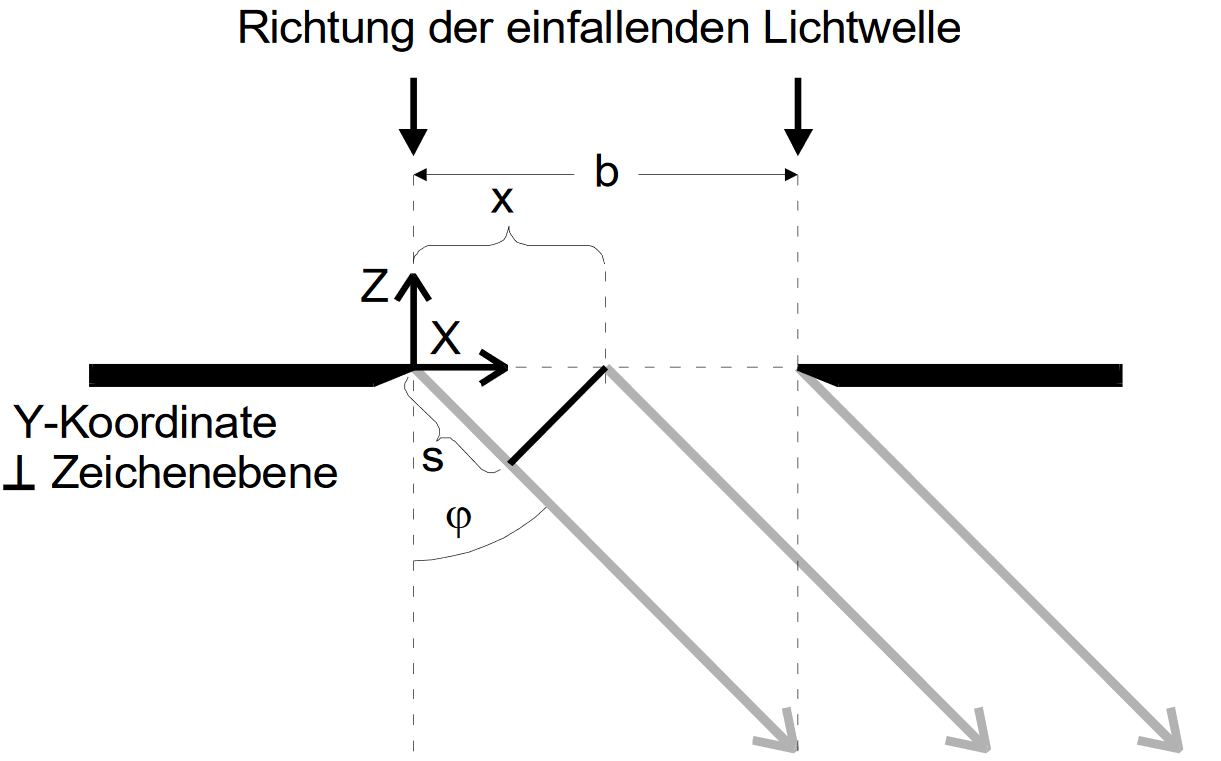
\includegraphics[width=\linewidth-150pt,height=\textheight-150pt,keepaspectratio]{content/images/Einzelspalt.png}
	\label{fig:Doppel}
\end{figure}
Beim einem N-fach Spalt mit gleichen Breiten $b$ und gleichen Abständen $d$ ergibt sich für die Welle nach Formel \eqref{eq:Integral} durch Superposition
\begin{equation}
\begin{split}
	\psi_\text{N} &=  C \sum\limits_{j=0}^{N-1} \int_{\mathbb{R}^2} F_1(x-x_j,y-y_j) \exp\left(-i k \hat{\vec{a}_0} \vec{x}\right) \diff x \diff y \\
	&= C \int_{\mathbb{R}^2} F_1(x',y') \exp\left(-i k \hat{\vec{a}_0} \vec{x}'\right) \diff x' \diff y'  \sum\limits_{j=0}^{N-1} \exp\left(-i k \frac{a_1}{|\vec{a}_0|} j d \right) \\
	&= \psi_1 S,
\end{split}
\end{equation}
wobei $F_1(x,y)$ die Blendenfunktion von einem Einzelspalt und $S$ der Formfaktor ist.
Für die Intensität beim N-fach Spalt gilt somit
\begin{equation}
	I_\text{N} = I_1 S^2 \propto \frac{\sin^2(b \eta')}{(b\eta')^2}\frac{\sin^2(N d \eta')}{\sin^2(d\eta')}
\end{equation}
mit
\begin{equation}
	\eta'=\frac{1}{2} \sin(\varphi) k.
\end{equation}

